
\chapter{Methodology}\label{chap:Methodology}


\section{Configuration}\label{sec:2-spec}
In this experimental setup, two fundamental sensors are employed to acquire and analyze data.
The Realsense D435i camera, 
known for its high-resolution image capture and depth-sensing capabilities, is utilized for visual data acquisition. 
Complementing the camera is the AWR1843boost mmWave radar, operating in the 77-81GHz frequency range. 
Both sensors are securely housed within a custom 3D-printed enclosure as seen in figure \ref{fig:radar_camera_setup_fig}, 
which not only safeguards them but also minimizes external interference, ensuring the integrity of data acquisition. 
The mmWave radar config that is used is a 77-81GHz chirp, with settings balanced between range and resolution,
collecting data at 20 frames per second.

\begin{figure}[hpbt]
    \centering
    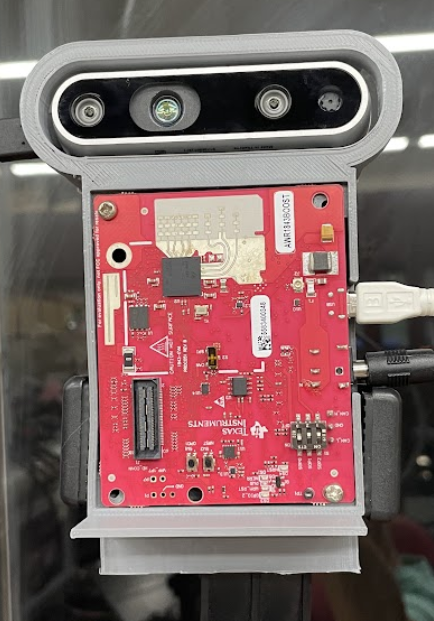
\includegraphics[width=5cm]{Figures/radar_camera_setup.png}%\textwidth
    \caption{Radar camera setup}
    \label{fig:radar_camera_setup_fig}
\end{figure}


\section{Overview}\label{sec:2-overview}
Overview block diagram of the algorithm shown in figure \ref*{fig:kf_update}.
\begin{figure}[hpbt]
    \centering
    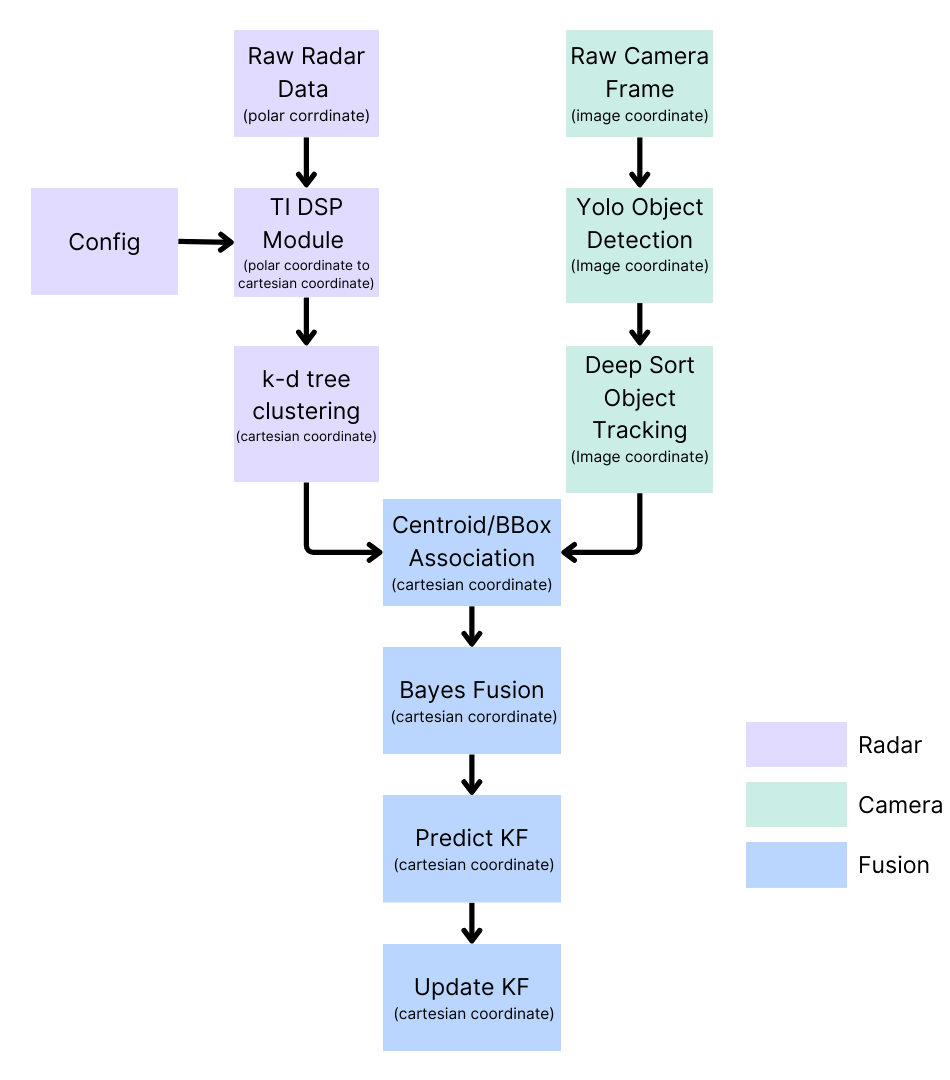
\includegraphics[width=10cm]{Figures/kf_update-modified.png}%\textwidth
    \caption{Radar camera Kalman Filter workflow}
    \label{fig:kf_update}
\end{figure}

\section{Calibration}\label{sec:2-calibration}
\subsection{Camera Calibration}
To accurately map the monocular camera's image coordinates to real-world coordinates, calibration of intrinsic and extrinsic is required.
Using tools provided by ROS \cite{cam_calib} as shown in figure \ref*{fig:camera_calibration}.

\begin{figure}[hpbt]
    \centering
    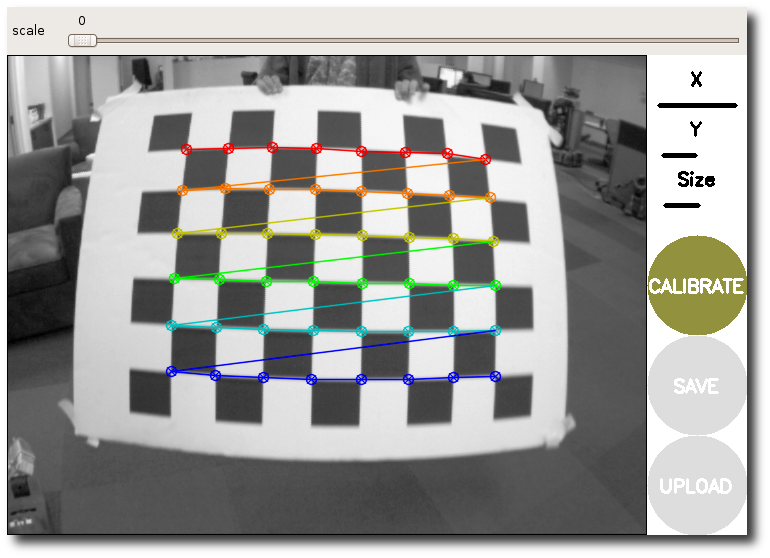
\includegraphics[width=6cm]{Figures/cam_calib.png}%\textwidth
    \caption{Camera extrinsic and intrinsic calibration}
    \label{fig:camera_calibration}
\end{figure}

\subsection{Radar-Camera Calibration}
In order to achieve accurate sensor fusion, it is essential to conduct proper calibration of the two sensors. 
For this purpose, a corner reflector is employed (figure \ref*{fig:radar_camera_calibration} \subref{subfig:corner_reflector_fig}), primarily due to its strong radar reflection characteristics(white point in figure \ref*{fig:radar_camera_calibration} \subref{subfig:radar_view_fig}). 
Additionally, it offers the advantage of appearing as a single point in both radar and camera data, effectively reducing ambiguity (figure \ref*{fig:radar_camera_calibration} \subref{subfig:camera_view_fig}).

Data points from both radar and camera coordinates can be collected with the corner reflector positioned at various locations.
After data is collected, radar points are associated with image points based on equation \ref*{equ:img2cart}
\begin{figure}[hbpt]
    \centering
    \begin{subfigure}{0.25\linewidth}
        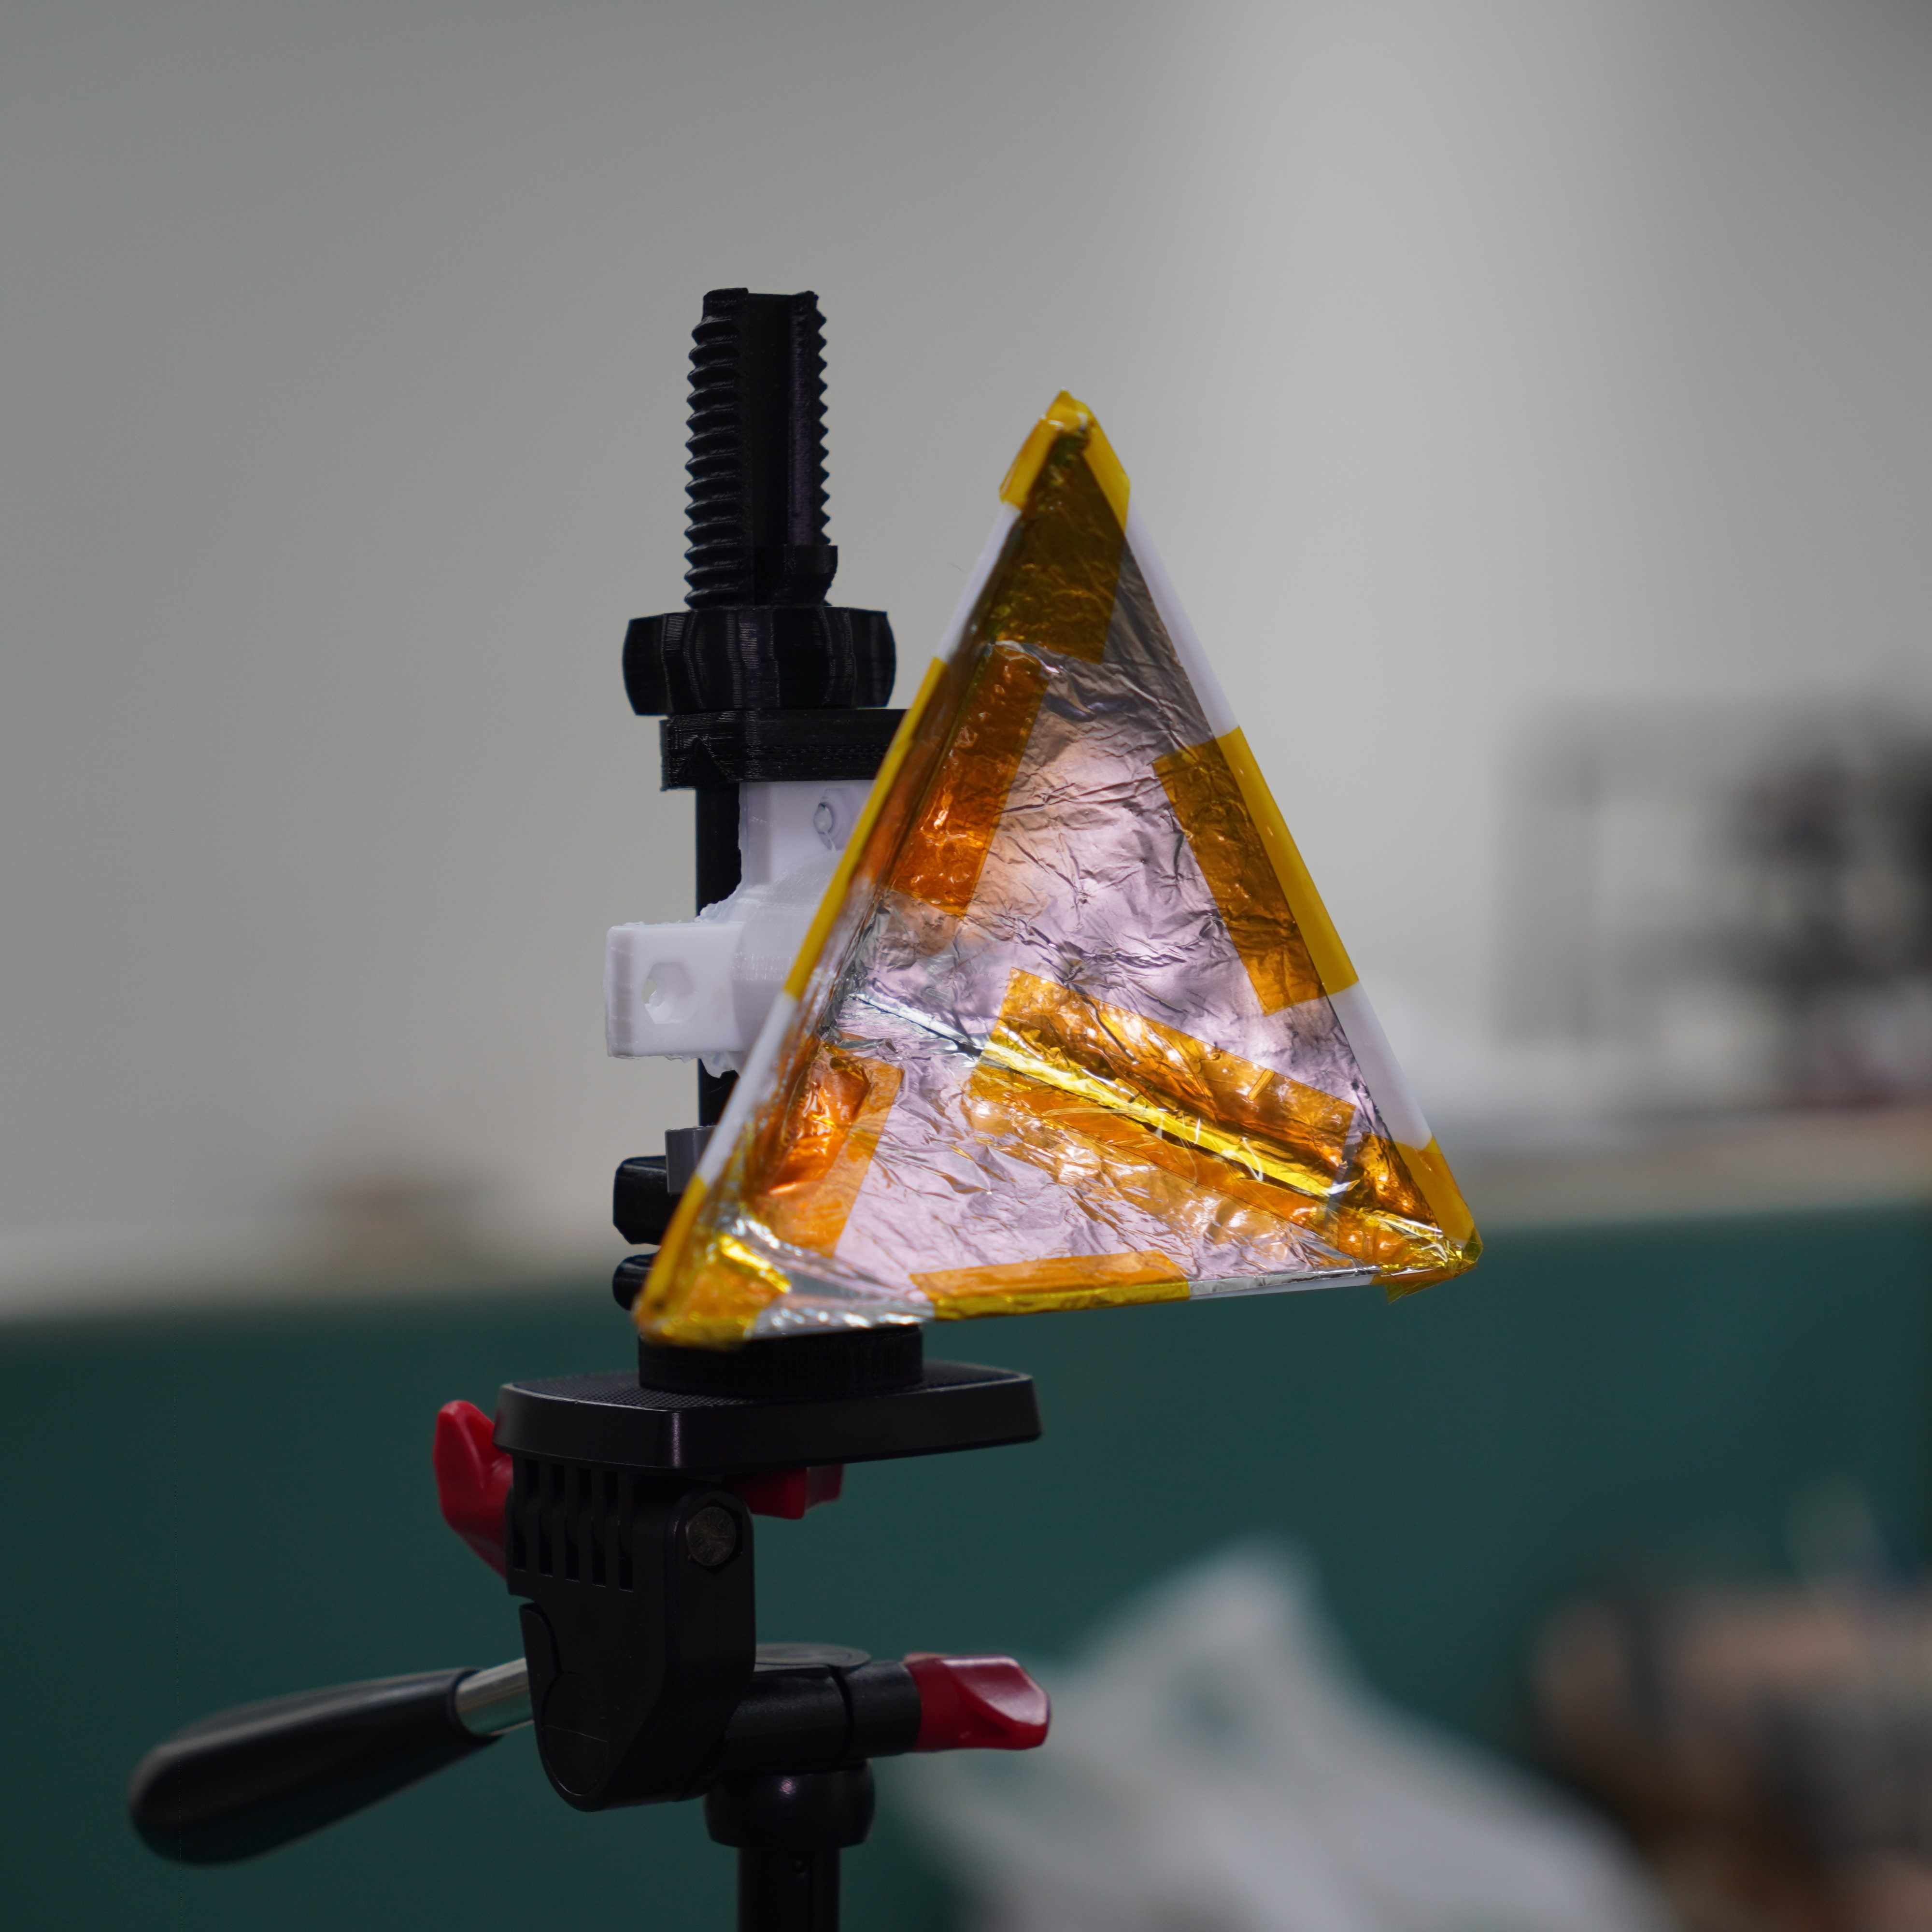
\includegraphics[width=5.5cm]{Figures/corner_reflector.jpg}
        \caption{Radar Corner Reflector}
        \label{subfig:corner_reflector_fig}
    \end{subfigure}
    \hfill
    \begin{subfigure}{0.25\linewidth}
        \centering
        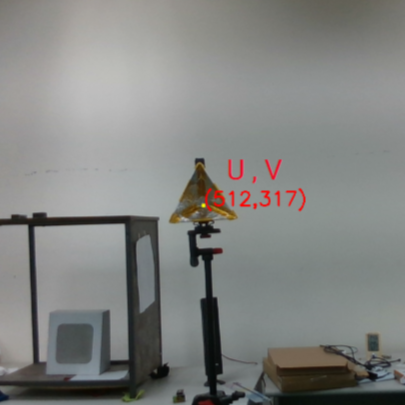
\includegraphics[width=5.5cm]{Figures/camera_corner.png}
        \caption{Camera-corner reflector calibration}
        \label{subfig:camera_view_fig}
    \end{subfigure}
    \hfill
    \begin{subfigure}{0.25\linewidth}
        \centering
        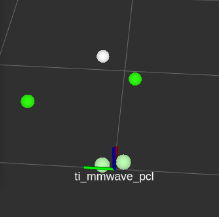
\includegraphics[width=5.5cm]{Figures/radar_corner.png}
        \caption{Radar-corner reflector calibration}
        \label{subfig:radar_view_fig}
    \end{subfigure}

    \caption{Radar camera calibration}
    \label{fig:radar_camera_calibration}
\end{figure}

\section{Data Pre-Processing}\label{sec:2-preprocessing}
\subsection{mmWave Radar Data Pre-Processing}\label{sec:2-kd_tree}
Given that radar data is inherently sparse and noisy, its data needed to be filtered.
For this purpose, k-d tree is employed to cluster the pointcloud.
A k-d tree, short for k-dimensional tree, is a hierarchical data structure used for efficient multidimensional data organization and search operations. 
It arranges data points in k-dimensional space, such as spatial coordinates, in a binary tree structure. 

\subsection{Image Data Pre-Processing}\label{sec:2-img_recognition}
\subsubsection{Image Recognition and Tracking\small(to be done)}
YOLOv3 is utilized to generate bounding boxes (BBox) and regions of interest (ROI)\cite{redmon2018yolov3}.
Subsequently, DeepSORT is applied for tracking the generated bounding boxes, 
enabling robust and efficient object tracking throughout the analysis\cite{Wojke2017simple}.

\subsubsection{Image to Real-world projection}
Before fusing, the detection results need to be converted into cartesian coordinates.

Conversion image to real-world vector, seen in figure \ref{fig:camera_projection}.
\begin{equation}\label{equ:img2cart}
u=c_x-\frac{p_x}{p_y}f
\end{equation}
where
\begin{align*}
    c_x &=\text{center of camera image in pixel}\\
    p_x &=\text{x-axis position in cartesian}\\
    p_y &=\text{y-axis position in cartesian}\\
    f &=\text{camera focal length in pixel}\\
    u &=\text{center of Bbox object detection in pixel}
\end{align*}

From equation \ref{equ:img2cart} we can obtain
\begin{equation}\label{equ:2_img2cart2}
    u=640-\frac{p_x}{p_y}950
\end{equation}

Thus
\begin{equation}\label{equ:2_cam_px}
    p_{x_{cam}}=
    \frac
    {(640-u)p_{y_{radar}}}
    {950}
\end{equation}


\begin{table}[htbp]
    \centering
    \begin{tabular}{|c|c|c|c|c|c|}
    \hline
    \textbf{u} & \textbf{v } & \textbf{range } & \textbf{azimuth} & \textbf{$p_{x_{cam}}$ (from eq \ref{equ:2_cam_px})} & \textbf{abs error} \\ 
    (pixel)   &(pixel)&(m)&ground truth(m)&(m)&(m)\\
    \hline
    639 & 297 & 1.002969742 & 0.0313581191 & 0.001055757623 & 0.03030236148 \\ \hline
    589 & 299 & 1.045041323 & 0.06544303149 & 0.05610221838 & 0.009340813113 \\ \hline
    564 & 303 & 1.042476892 & 0.09816454351 & 0.0833981514 & 0.01476639211 \\ \hline
    493 & 304 & 1.028517962 & 0.196329087 & 0.1591496214 & 0.03717946561 \\ \hline
    433 & 306 & 1.013839126 & 0.261772126 & 0.2209102095 & 0.04086191648 \\ \hline
    356 & 307 & 0.9946479797 & 0.3272151649 & 0.297347396 & 0.02986776885 \\ \hline
    240 & 317 & 1.03652215 & 0.4608280063 & 0.436430379 & 0.0243976273 \\ \hline
    200 & 315 & 1.020024657 & 0.496276319 & 0.4724324728 & 0.0238438462 \\ \hline
    100 & 316 & 1.057939529 & 0.6108016372 & 0.6013551009 & 0.00944653624 \\ \hline
    23 & 321 & 1.071923614 & 0.6721544862 & 0.6961861785 & 0.0240316923 \\ \hline
    973 & 230 & 0.6216549873 & -0.2045094818 & -0.2179064324 & 0.01339695062 \\ \hline
    945 & 241 & 0.6698815227 & -0.1963291019 & -0.2150672257 & 0.01873812377 \\ \hline
    885 & 270 & 0.8026226759 & -0.2072362751 & -0.2069921638 & 0.0002441112932 \\ \hline
    848 & 293 & 1.028517962 & -0.196329087 & -0.225191301 & 0.02886221403 \\ \hline
    801 & 318 & 1.422063112 & -0.2249604315 & -0.2410022748 & 0.01604184336 \\ \hline
    390 & 272 & 0.7117491364 & 0.2085996717 & 0.1873024043 & 0.02129726739 \\ \hline
    432 & 281 & 0.8026226759 & 0.2072362751 & 0.1757321227 & 0.03150415235 \\ \hline
    467 & 289 & 0.8514408469 & 0.1908755153 & 0.1550518595 & 0.03582365585 \\ \hline
    461 & 299 & 0.9365850091 & 0.2099630684 & 0.1764723333 & 0.03349073507 \\ \hline
    485 & 313 & 1.114227772 & 0.2126898468 & 0.1817950575 & 0.03089478926 \\ \hline
    512 & 317 & 1.16350615 & 0.1840585321 & 0.1567671445 & 0.02729138766 \\ \hline
    515 & 328 & 1.422063112 & 0.2249604315 & 0.1871135674 & 0.03784686405 \\ \hline
    533 & 330 & 1.428454399 & 0.1799683422 & 0.1608890744 & 0.019079 \\
    \hline
\end{tabular}
\caption{Real-world camera data converted to cartesian compared to real radar data}
\label{tab:data}
\end{table}

\begin{table}[h!]
    \begin{center}
      \label{tab:table4}
      \begin{tabular}{l|c} % <-- Alignments: 1st column left, 2nd middle and 3rd right, with vertical lines in between
        \textbf{Method} & \textbf{RMSE} \\% %object detected
        \hline
        Proposed                            & 0.0271 m \\%& 6m 
        \citeauthor{8794186}\cite{8794186} & 0.018 m \\%
        
      \end{tabular}
    \end{center}
    \caption{callibration method RMSE compared}
    \label{tab:callib_rmse}
  \end{table}

\begin{figure}[hpbt]
    \centering
    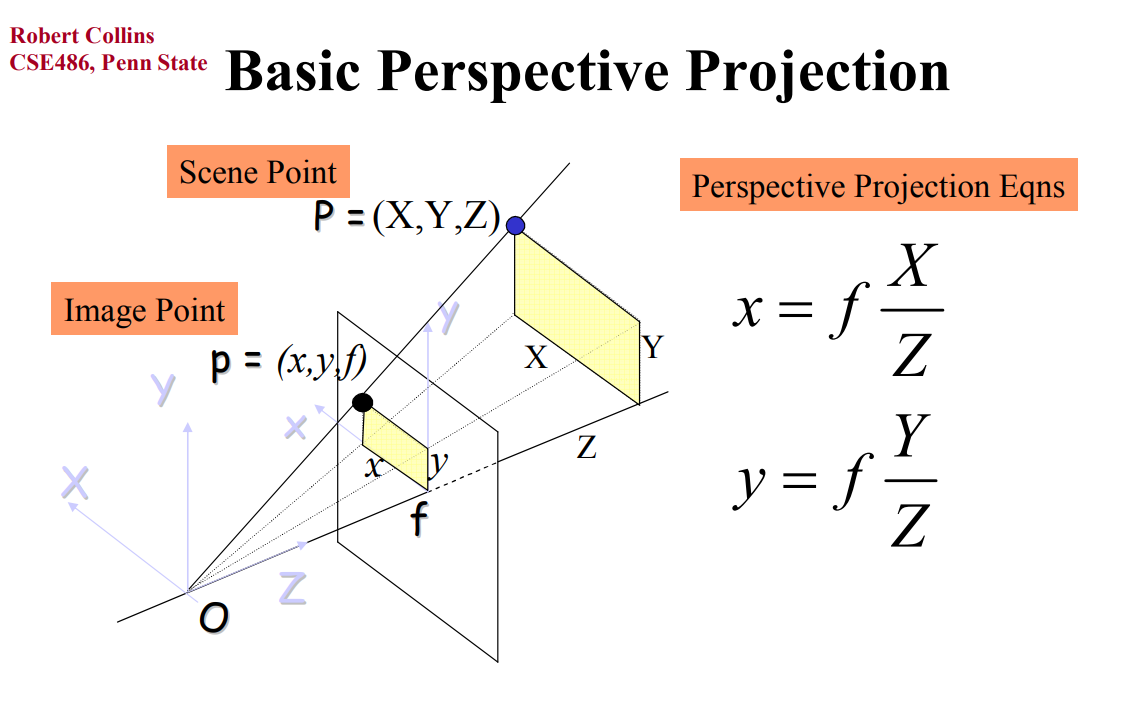
\includegraphics[width=8cm]{Figures/cam_projection.png}%\textwidth
    \caption{Camera to real-world projection}
    \label{fig:camera_projection}
\end{figure}
\newpage
\section{Radar-camera Data Association}\label{sec:2-association}
Before fusion, radar clusters have to be associated with tracked objects from deepsort.
First, centroids of radar clusters are mapped into image coordinates.
Second, is to find the theoretical error of radar's measurement \cite{8844649}, which is radar's resolution, determined by equation \ref*{equ:angular_resolution}
Finally, if the distance between the calculated radar centroid and the image detection lies within the theoretical boundary
, we can safely assume both measurements belong to the same object of interest.
\begin{equation}\label{equ:angular_resolution}
    \Delta \theta= \frac{c_0}{f_c d N_{RX} N_{TX} \cos(\theta _i)}
\end{equation}
where
\begin{align*}
    f_c & = \text{center frequency} \\
    \lambda & = \text{carrier signal wavelength} \\
    d & =  \lambda/2 \\
    N_{RX} & = \text{Number of receiving antenna}\\
    N_{TX}& = \text{Number of transferring antenna}\\
    \theta _i &= \text{angle of interest}
\end{align*}






